\documentclass[%
  a4paper,%
  11pt,% <10pt, 9pt>
  %style=screen,
  %sender=bottom,
  blue,% <orange, green, violet>
  %rgb, <cmyk>
  %mono,
  hyperref	% tubs color for hyperref
  ]{tubsartcl}
\usepackage[utf8]{inputenc}
\usepackage{hyperref}
\usepackage[english=british]{csquotes}
\usepackage{graphicx}
\usepackage{tikz}

\setlength{\parindent}{0cm}
 
% Titelseiten-Elemente
\title{TuringBrain IDE \LARGE 1.0}
\subtitle{User Guide}
\author{\small Vanessa Baier, Nils Breyer, Phillipp Neumann,\\ Sven Schuster, David Wille}
\logo{
\includegraphics{ips}}
\titleabstract{TuringBrain IDE -- User Guide}
\titlepicture{title}
% Rückseiten-Elemente
\address{
  Advisor: Matthias Hagner\\\\
  Technische Universität Braunschweig\\
  Institut für Programmierung und Reaktive Systeme\\
  Mühlenpfordtstr. 23\\
  38106 Braunschweig}
\backpageinfo{
}

\begin{document}

\maketitle[image,logo=right]%[<plain/image/imagetext>,<logo=left/right>]

\tableofcontents
\clearpage
\section{Introduction}

TuringBrain IDE allows you to develop and debug your own TuringMachines in an easy to use WYSIWYG (what you see is what you get) environment. It also enables you to program and run Brainfuck code.

\subsection{Features}

\begin{itemize}
  \item Edit Turing Machines by graphically editing the state graph
  \item Create Turing Machines with multiple tapes
  \item Write Brainfuck programs within the integrated code editor
  \item Simulate your machines and programs using the integrated simulation
  \item Simulate on special LEGO\textregistered -Tape (hardware needed), graphically animated on the screen or on the console
  \item Pause simulation, Debug step-by-step
  \item Live-highlighting of the current state and edge during the simulation
  \item Save machines as .tm (an XML-Format) respective .bf
  \item Copy \& Paste (just for transitions on edges), Undo \& Redo
  \item Export to \LaTeX , SVG, and PNG
  \item and many more features...
\end{itemize}

\section{Getting started}

\subsection{Installation}
\label{sec:installation}
If you don't want to use the LEGO\textregistered\, tapes, you only have to download the executable .jar file from our repository.
To use the LEGO\textregistered\, tapes you have to do following steps:
\begin{enumerate}
	\item Download Version 0.8.5beta of LeJos from \href{http://sourceforge.net/projects/lejos/files/lejos-NXJ/}{http://sourceforge.net/projects/lejos/files/lejos-NXJ/}
	\item Download JGraph from \href{http://www.jgraph.com/jgraph.html}{http://www.jgraph.com/jgraph.html}
	\item Unpack the archive to a folder where you have executive rights
	\item Download eclipse and install it
	\item Add our project as a new project in eclipse
	\item In eclipse open Window \textgreater\ Preferences and choose Java \textgreater\ Build Path \textgreater\ Classpath Variables
	\item Add two new Classpath Variables ``JGRAPH\_HOME'' and ``NXJ\_HOME'' pointing to the corresponding folder (e.g. figure \ref{pic:eclipse_preferences})
	\item In eclipse open Project \textgreater\ Properties and choose Java Build Path \textgreater\ Libraries and add following Libraries (figure \ref{pic:libraries}):
	\begin{enumerate}
	\item[$\bullet$] JGRAPH\_HOME/lib/jgraphx.jar
	\item[$\bullet$] NXJ\_HOME/3rdparty/lib/bcel.jar
	\item[$\bullet$] NXJ\_HOME/3rdparty/lib/bluecove-gpl.jar
	\item[$\bullet$] NXJ\_HOME/3rdparty/lib/bluecove.jar
	\item[$\bullet$] NXJ\_HOME/lib/classes.jar
	\item[$\bullet$] NXJ\_HOME/lib/jtools.jar
	\item[$\bullet$] NXJ\_HOME/lib/pccomm.jar
	\item[$\bullet$] NXJ\_HOME/lib/pctools.jar
	\end{enumerate}
	\item In eclipse open Run \textgreater\ External Tools \textgreater\ External Tools Configuration
	\item Now you add a rule in the field ``Program'' and name it ``lejos Compile'' and add in Main:
	\begin{enumerate}
	\item[$\bullet$] Location: [your lejos location]/bin/nxjc
	\item[$\bullet$] Working directory: \$\{project\_loc\}
	\item[$\bullet$] Arguments: -cp \textquotedbl .:[your lejos location]/lib/jgraphx.jar\textquotedbl\ \${resource\_loc}
	\end{enumerate}
	\item Now you add a rule in the field ``Program'' and name it ``lejos pc'' and add in Main:
	\begin{enumerate}
	\item[$\bullet$] Location: [your lejos location]/bin/nxjpc
	\item[$\bullet$] Working directory: \$\{project\_loc\}
	\item[$\bullet$] Arguments: -cp \textquotedbl .:[your lejos location]/lib/jgraphx.jar\textquotedbl\ \${java\_type\_name}
	\end{enumerate}
	\item Now you add a rule in the field ``Program'' and name it ``lejos pc Compile'' and add in Main:
	\begin{enumerate}
	\item[$\bullet$] Location: [your lejos location]/bin/nxjpcc
	\item[$\bullet$] Working directory: \$\{project\_loc\}
	\item[$\bullet$] Arguments: -cp \textquotedbl .:[your lejos location]/lib/jgraphx.jar\textquotedbl\ \${resource\_loc}
	\end{enumerate}
	\item Now you add a for every NXT module you want to use rule in the field ``Program'' and name it ``lejos Upload ([NXT module name])'' and add in Main:
	\begin{enumerate}
	\item[$\bullet$] Location: [your lejos location]/bin/nxj
	\item[$\bullet$] Working directory: \$\{project\_loc\}
	\item[$\bullet$] Arguments: \${java\_type\_name} -v -n [NXT module name] -r -b
	\end{enumerate}
	\item Now you have to add these rules to the favorites, so you can run them from the external tools run button in the menubar. Simply go to Run\ \textgreater\ External Tools \textgreater\ Organize Favorites and add the rules you need.
\end{enumerate}

\begin{figure}[!htb]
\begin{center}
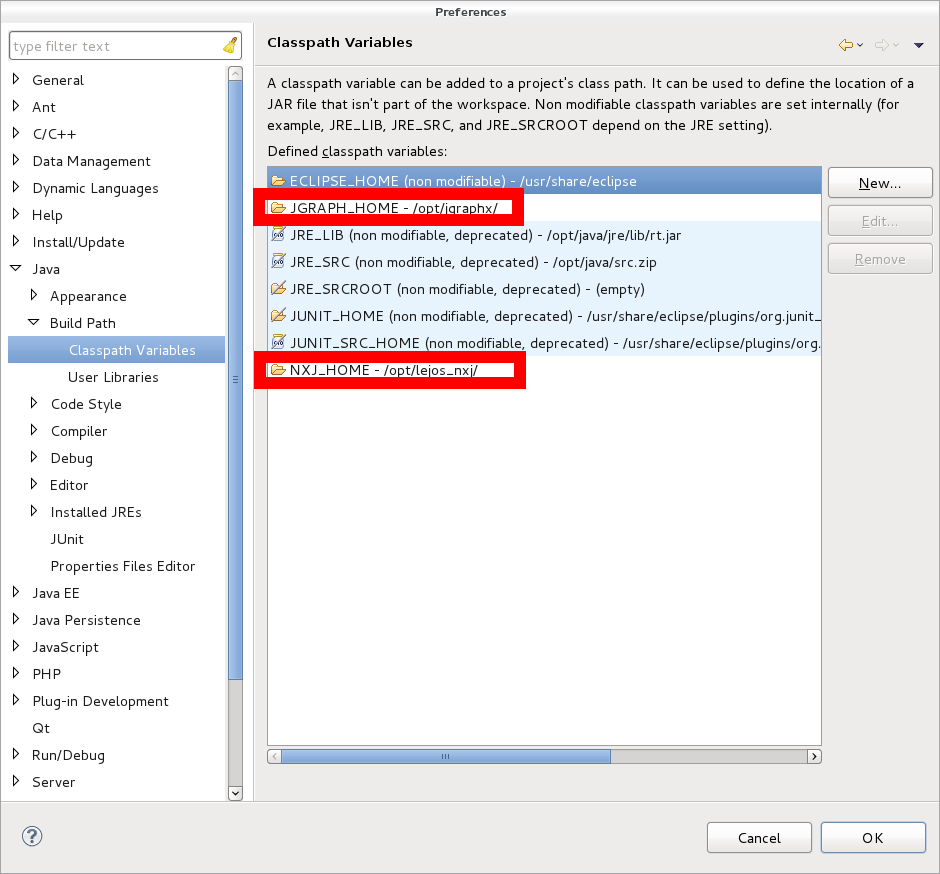
\includegraphics[scale=0.45]{graphics_install/eclipse_preferences.png}
\end{center}
\caption{Eclipse preferences}
\label{pic:eclipse_preferences}
\end{figure}

\begin{figure}[!htb]
\begin{center}
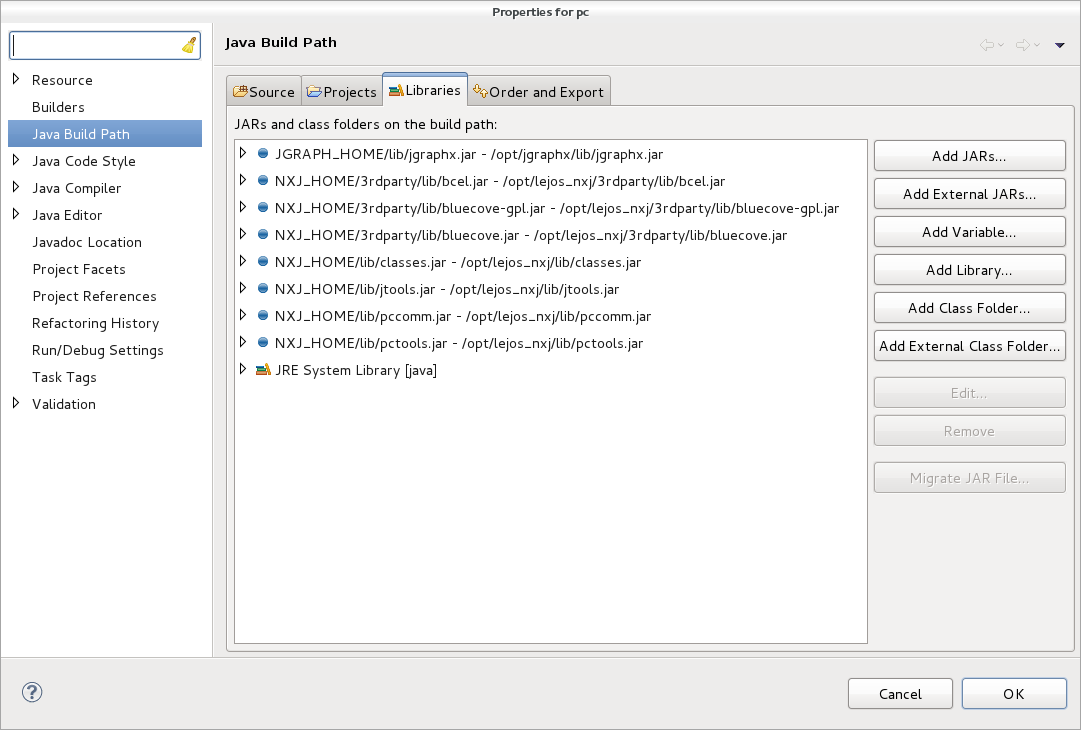
\includegraphics[scale=0.45]{graphics_install/libraries.png}
\end{center}
\caption{Libraries}
\label{pic:libraries}
\end{figure}

\clearpage

\subsection{Welcome page}
\label{sec:welcome-page}
If the installation was correct and you have started the application the one or the other way you will see the welcome page like in figure \ref{pic:welcome_page}. Now you can open a turing machine, create a new one or open an example that is listed below. \\
You can also do the same with brainfuck applications.
\begin{figure}[!htb]
\begin{center}
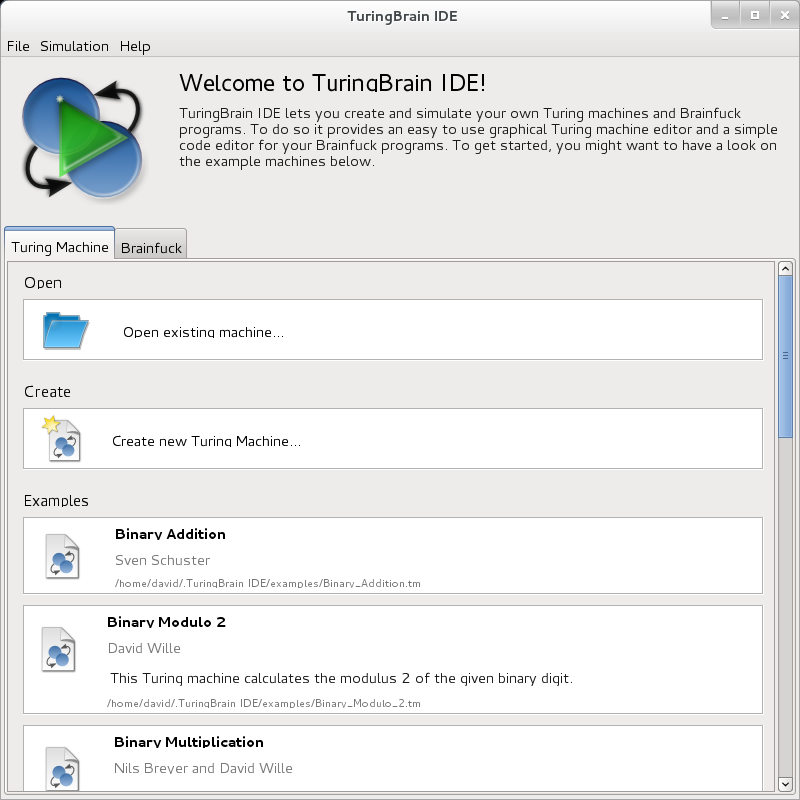
\includegraphics[scale=0.45]{graphics_gui/welcomescreen.png}
\end{center}
\caption{Welcome page}
\label{pic:welcome_page}
\end{figure}

\clearpage

\section{Turing Machine editor}
Creating a new machine (via the menu or the welcome page) first leads to a dialog that lets you set the name of the machine and the number of tapes.

\textbf{Important:} The number of tapes is set when creating the Turing machine. It cannot be changed afterwards!

If you open an example or another existing machine you will see a window like figure \ref{pic:turing_editor}. If you have created a new machine the graph will be empty. On the left side you see a toolbox (\ref{sec:toolbox}) and also panels will be displayed to change the properties of the machine and all its components.
\begin{figure}[!htb]
\begin{center}
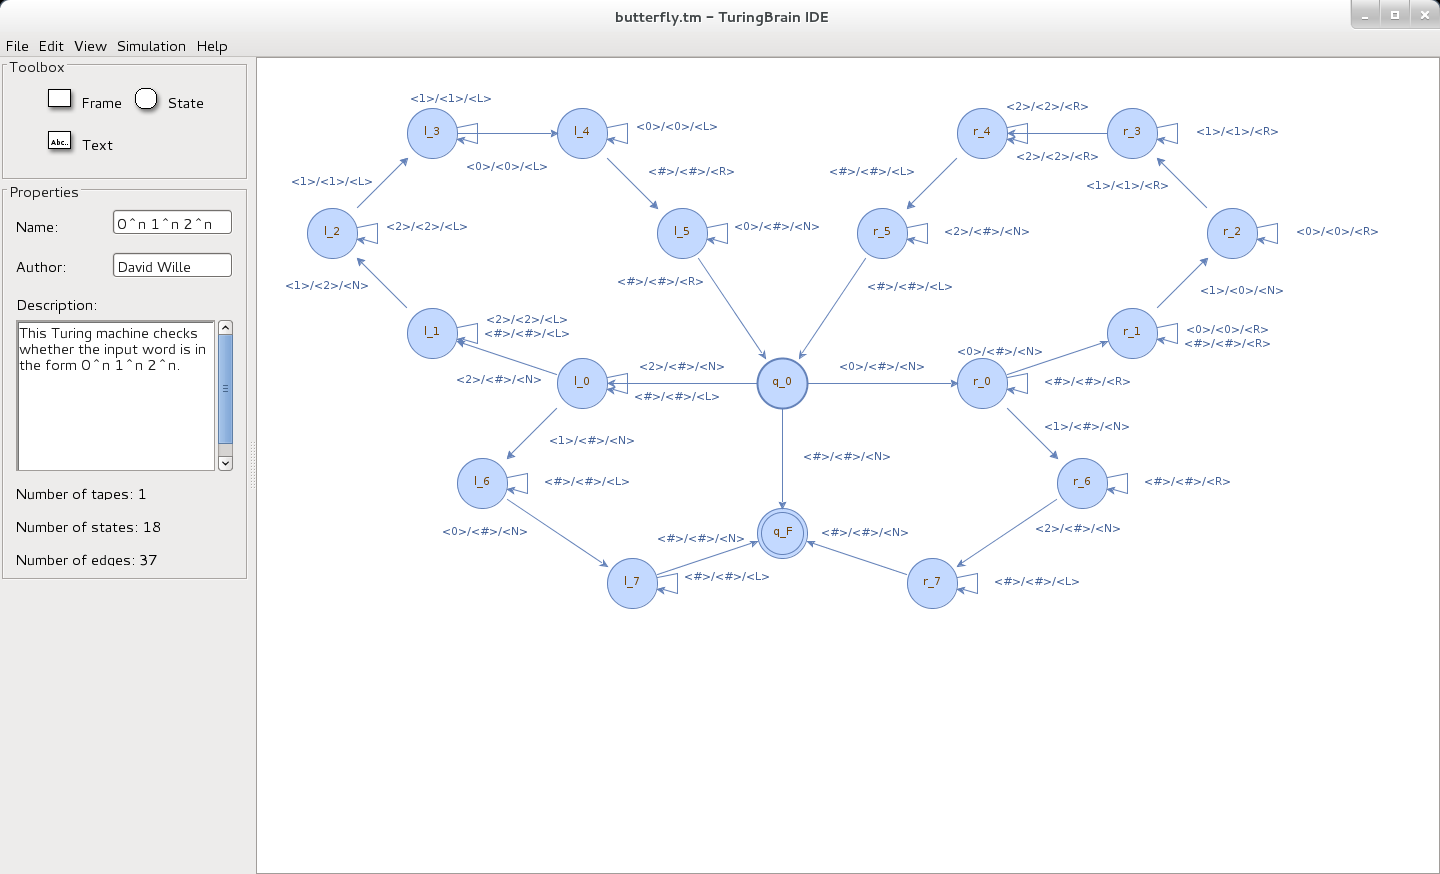
\includegraphics[scale=0.3]{graphics_gui/turing_editor.png}
\end{center}
\caption{Turing Machine editor}
\label{pic:turing_editor}
\end{figure}

\subsection{Toolbox}
\label{sec:toolbox}
With the toolbox you can use drag an drop to add states, frames and textboxes to your machine. While states have a fixed size, frames and textboxes can be resized.
\begin{figure}[!htb]
\begin{center}
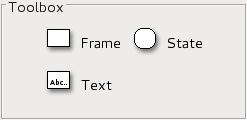
\includegraphics[scale=0.5]{graphics_gui/toolbox_turing.png}
\end{center}
\caption{Toolbox}
\label{pic:toolbox}
\end{figure}

\clearpage

\subsection{Edit machine properties}
\label{sec:edit-mach-prop}
First of all you should edit the turing machine properties and enter an author and a description. These fields don't are entirely optional, but they can help to organize and document your machines. In the machine properties you will also see some statistics about your machine like the number of states.
\begin{figure}[!htb]
\begin{center}
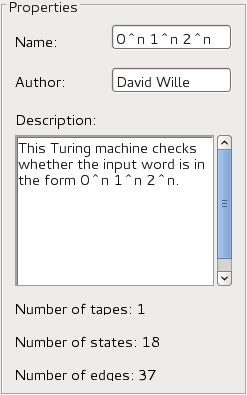
\includegraphics[scale=0.5]{graphics_gui/machine_properties.png}
\end{center}
\caption{Edit machine properties}
\label{pic:machine_properties}
\end{figure}

\subsection{Adding and changing states}
\label{sec:add-edit-states}
If you have created or selected a state you can change the properties of the selected state. You can specify the label or whether it is a start and/or final state. The start state will be marked with a bold border and the final will be marked with a double circle.

\textbf{Important:} Every Turing machine must have exactly one state marked as start state. Having multiple start states leads to undefined behaviour, having no start state will lead to an error when simulating.


\begin{figure}[!htb]
\begin{center}
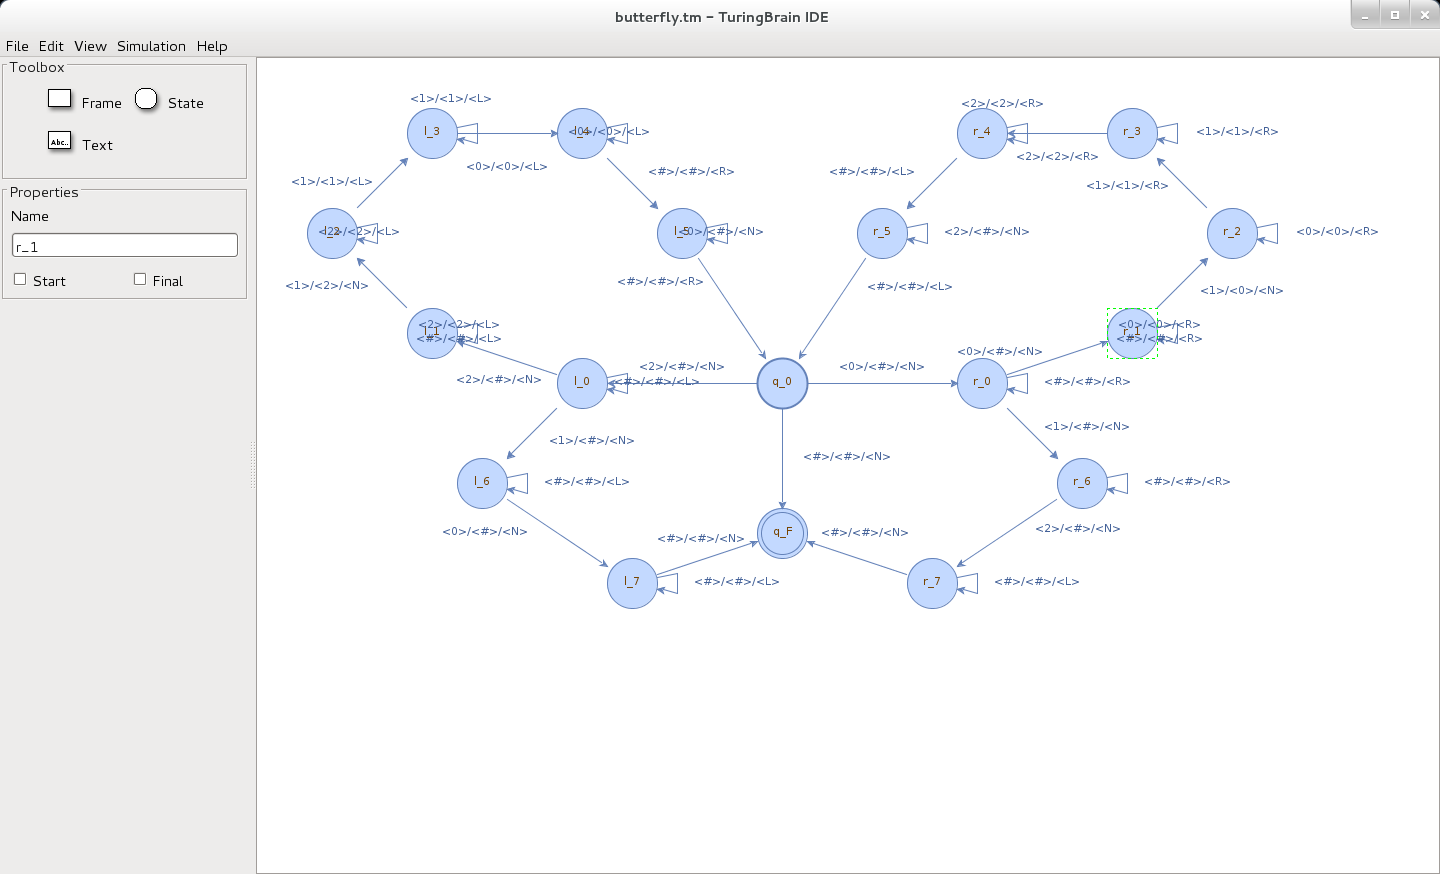
\includegraphics[scale=0.5]{graphics_gui/state_properties.png}
\end{center}
\caption{Adding and changing states}
\label{pic:state_properties}
\end{figure}

\clearpage

\subsection{Adding and changing edges}
\label{sec:adding-chang-edges}
If you want to create an edge you have to move the mouse pointer to the center of a state, which will be highlighted with a bold green square. Then you have to hold the left mouse button and drop the arrow on the state where the edge shall end. \\
If you have selected an edge you can add, remove or edit transitions. If you want to edit a transition you just have to double click on it.
\begin{figure}[!htb]
\begin{center}
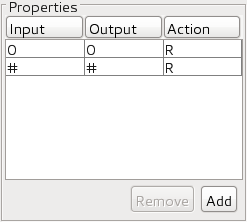
\includegraphics[scale=0.5]{graphics_gui/edge_properties.png}
\end{center}
\caption{Adding and changing edges}
\label{pic:edge_properties}
\end{figure}

\subsection{Edit transitions}
\label{sec:edit-transitions}
If you double clicked on a transtion or added a new one, you can edit it. Every transition specifies an input (the read symbol), an output (the symbol to write) and an action (movment of the head) individually for every tape. The transition is executed only, if all input symbols on all tapes match. If they match, the transition is always completly executed (on all tapes).
\bigskip

\emph{Input.} Every character can be used as an input symbol, except for *, which is a wildcard. The * always matches, regardless of the read symbol.

\emph{Output.} Again every character can be used as an output symbol, except for * which has a special meaning. The * reproduces the read symbol (it never changes it).

\emph{Action.} Allowed actions are: \emph{L} (moves the head one field to the left), \emph{R} (moves the head one filed to the right) and \emph{N} (does nothing).
\bigskip

\textbf{Important:}  For LEGO\textregistered\, tapes, allowed input and output characters are only \#, 0, 1, 2 and *, otherwise the simulation will stop with an error message.

If you don't want to use every tape in a transition, use the combination */*/N as input/output/action, this will reproduces the exisiting symbol and let the head stay where it is. In fact this setting is the default when you add a new transition, so you only have to change the tapes you want to use in the transition.

\textbf{Important:} Make sure that only the input conditions of one transition per state can be met at a time. Using multiple transitions with * input symbols or with identical inputs can lead to undeterministic behaviour.


\begin{figure}[!htb]
\begin{center}
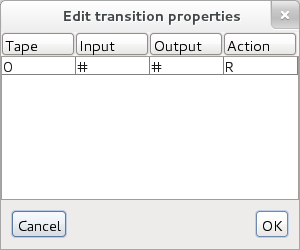
\includegraphics[scale=0.5]{graphics_gui/edit_transitions.png}
\end{center}
\caption{Edit transitions}
\label{pic:edit_transitions}
\end{figure}

\clearpage

\subsection{Via points}
\label{sec:via-points}
Sometimes it is useful to set via points for edges. For example, if the direct way crosses other states or edges. For this case TuringBrainIDE supports to set via points for edges, to set the way of the edge manually. These via points don't affect the simulation at all and are only a tool for better visualisation. When you select an edge you can add via points with Edit \textgreater \ Add via point.

\subsection{Frames and textboxes}
\label{sec:frames-textboxes}
As via points frames and textboxes don't affect the simulation. These tools provide you a simple way to structure, comment and document your machines. In the property panel of a textbox you can change the text to be displayed.
\begin{figure}[!htb]
\begin{center}
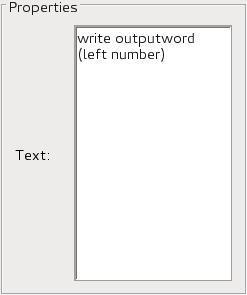
\includegraphics[scale=0.5]{graphics_gui/text_properties.png}
\end{center}
\caption{Textbox properties}
\label{pic:text_properties}
\end{figure}

\subsection{Export}
\label{sec:export}
In the menu File \textgreater \ Export you can export the turing machine as a table to \LaTeX\ (.tex), or as a graphic to Scalable Vector Graphic (.svg) or Portable Network Graphic (.png)

The export to \LaTeX\ generates a document with tables containing all transitions, the SVG and PNG exporters export the graph as you see it in the editor.

\textbf{Important:} The \LaTeX\ exporter copies the state names, machine name etc. as you entered them in the machine. There might be problems with characters you have to escape in \LaTeX. 

\clearpage

\section{Brainfuck editor}
\label{sec:brainfuck-editor}
The Brainfuck editor  can be used to create applications using the esoteric programming language brainfuck. Our brainfuck interpreter differs a little from the original brainfuck implementation. Instead of an array of ASCII-symbols, we use a TuringMachine tape (Action) providing only the symbols \#, 0, 1, 2 with $\# < 0 < 1 < 2$. Also the input and output strings are replaced by the tapes Input and Output.\\

The brainfuck language consists of only eight commands, each consisting of only one character:\\

\begin{tabular}{|c|l|}
\hline
\textbf{Command} & \textbf{Meaning} \\
\hline
$>$ & move to the next symbol on Action tape \\
\hline
$<$ & move to the previous symbol on Action tape \\
\hline
+ & increment symbol at current position on Action tape \\
\hline
-- & decrement symbol at current position on Action tape \\
\hline
. & output symbol at current position on Action tape, symbol is written on Output tape \\
\hline
, & read next symbol from Input tape, write it to the current position on Action tape \\
\hline
[ & if current symbol is a \#, move to corresponding ] command, else execute following\\
\ & commands \\
\hline
] & if current symbol is not a \#, jump back to corresponding [ command \\
\hline
\end{tabular}

\bigskip
The commands are executed sequentially. Every other character within the code will be ignored.An example can be seen in figure \ref{pic:brainfuck_editor}.

\begin{figure}[!htb]
\begin{center}
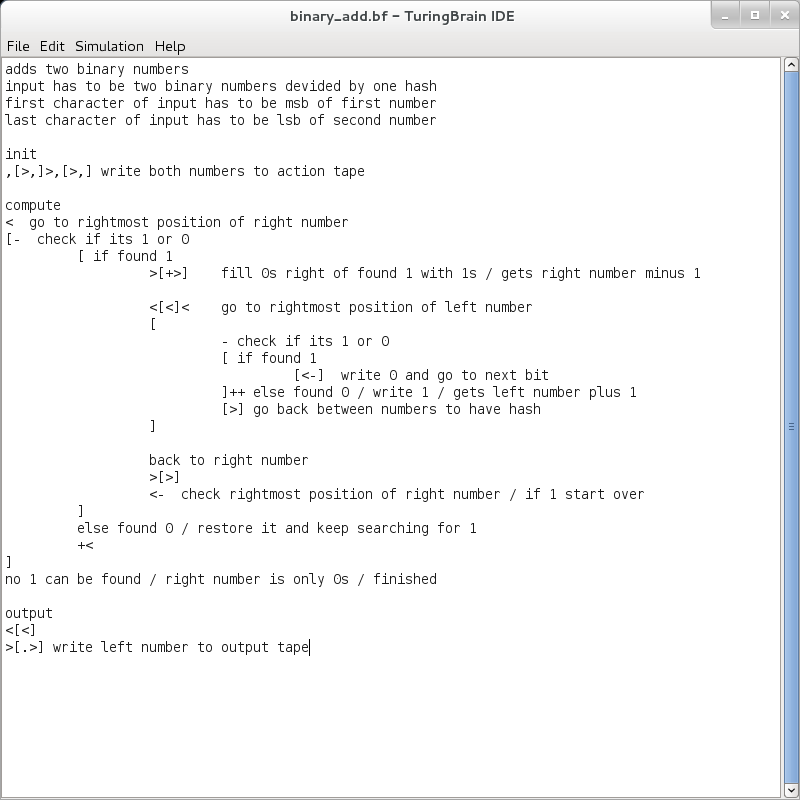
\includegraphics[scale=0.5]{graphics_gui/brainfuck_editor.png}
\end{center}
\caption{Brainfuck editor}
\label{pic:brainfuck_editor}
\end{figure}

\clearpage

\section{Run window}
In the Input tab (Figure \ref{pic:run_window_input}) of the run window you can specify the input word for every tape. In the tape settings tab (Figure \ref{pic:run_window_tape_settings}) you can specify a label for every tape and the type of the tape. If you choose a LEGO\textregistered\, Tape you should specify the main and the slave robots for the tapes in the Robot settings tab. With run you can start the presimulation.
\begin{figure}[!htb]
\begin{center}
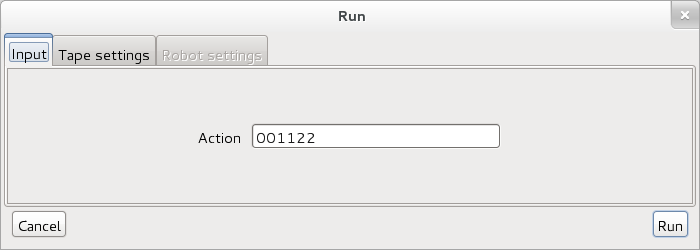
\includegraphics[scale=0.5]{graphics_gui/run_window_input.png}
\end{center}
\caption{Run window -- Input}
\label{pic:run_window_input}
\end{figure}


\begin{figure}[!htb]
\begin{center}
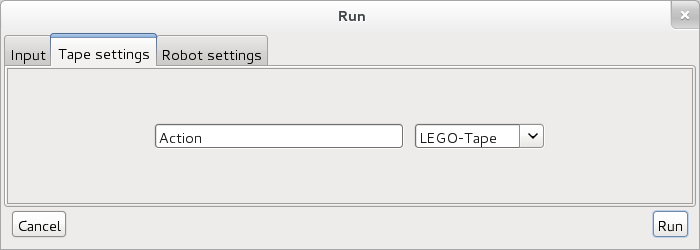
\includegraphics[scale=0.5]{graphics_gui/run_window_tape_settings.png}
\end{center}
\caption{Run window -- Tape settings}
\label{pic:run_window_tape_settings}
\end{figure}


\begin{figure}[!htb]
\begin{center}
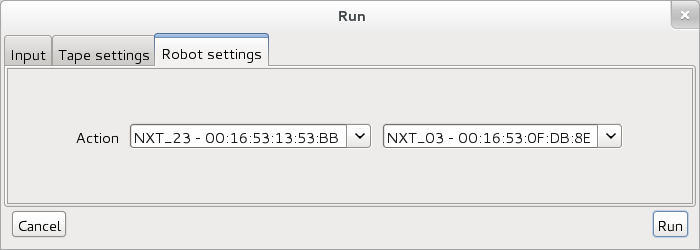
\includegraphics[scale=0.5]{graphics_gui/run_window_robot_settings.png}
\end{center}
\caption{Run window -- Robot settings}
\label{pic:run_window_robot_settings}
\end{figure}
 
\section{Simulation}

\subsection{Organize robots}
In the menu Simulation \textgreater\ Organize robots you can add the robots with their hardware address and define if the corresponding robot is a master module.
\begin{figure}[!htb]
\begin{center}
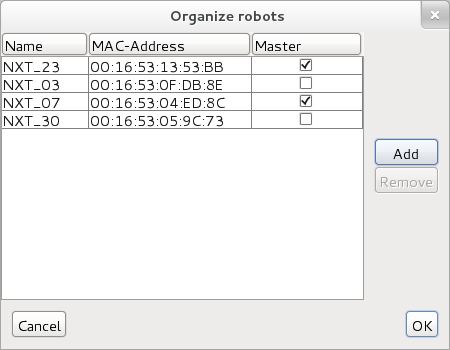
\includegraphics[scale=0.45]{graphics_gui/organize_robots.png}
\end{center}
\caption{Organize robots}
\label{pic:organize_robots}
\end{figure}

\subsection{Presimulation window}
The Presimulation window (Figure \ref{pic:presimulation}) shows the estimated duration of the simulation. It also displays a warning if the simulation could be too long.
\begin{figure}[!htb]
\begin{center}
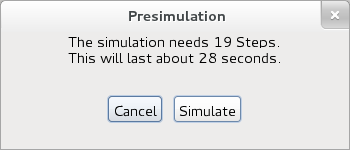
\includegraphics[scale=0.4]{graphics_gui/presimulation.png}
\end{center}
\caption{Presimulation window}
\label{pic:presimulation}
\end{figure}

\subsection{Simulation window}
If you run the simulation after the presimulation you will see the turing machine and the tapes (Figure \ref{pic:simulation_window}). After the input word has been written you can start the simulation with the play button. If you have paused the simulation you can simulate the next step with the second button. If you simulate on the LEGO\textregistered\, Tape you can mute and unmute the sound.
\begin{figure}[!htb]
\begin{center}
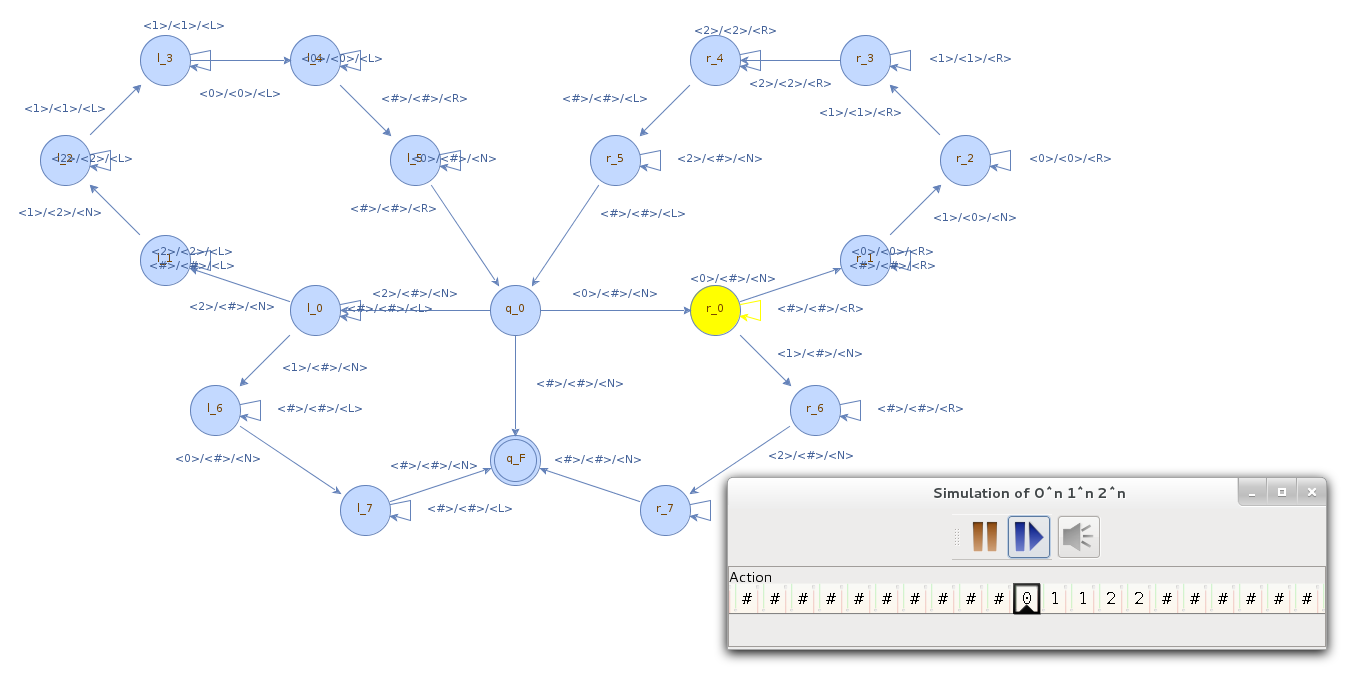
\includegraphics[scale=0.35]{graphics_gui/simulation_window.png}
\end{center}
\caption{Simulation window}
\label{pic:simulation_window}
\end{figure}

\clearpage

\section{Hardware -- LEGO\textregistered\, tape}

This section describes the position of the components used in the machine. The following subsections and pictures are meant to extend the building instructions file created with the LEGO\textregistered\, Digital Designer.

\subsection{The machine's motor section}

Figure \ref{pic:topview} shows a view of the machine's motor section to get a brief overview of it's position and the number 1 -- 4 represent the following pictures.

\begin{figure}[!htb]
\begin{center}
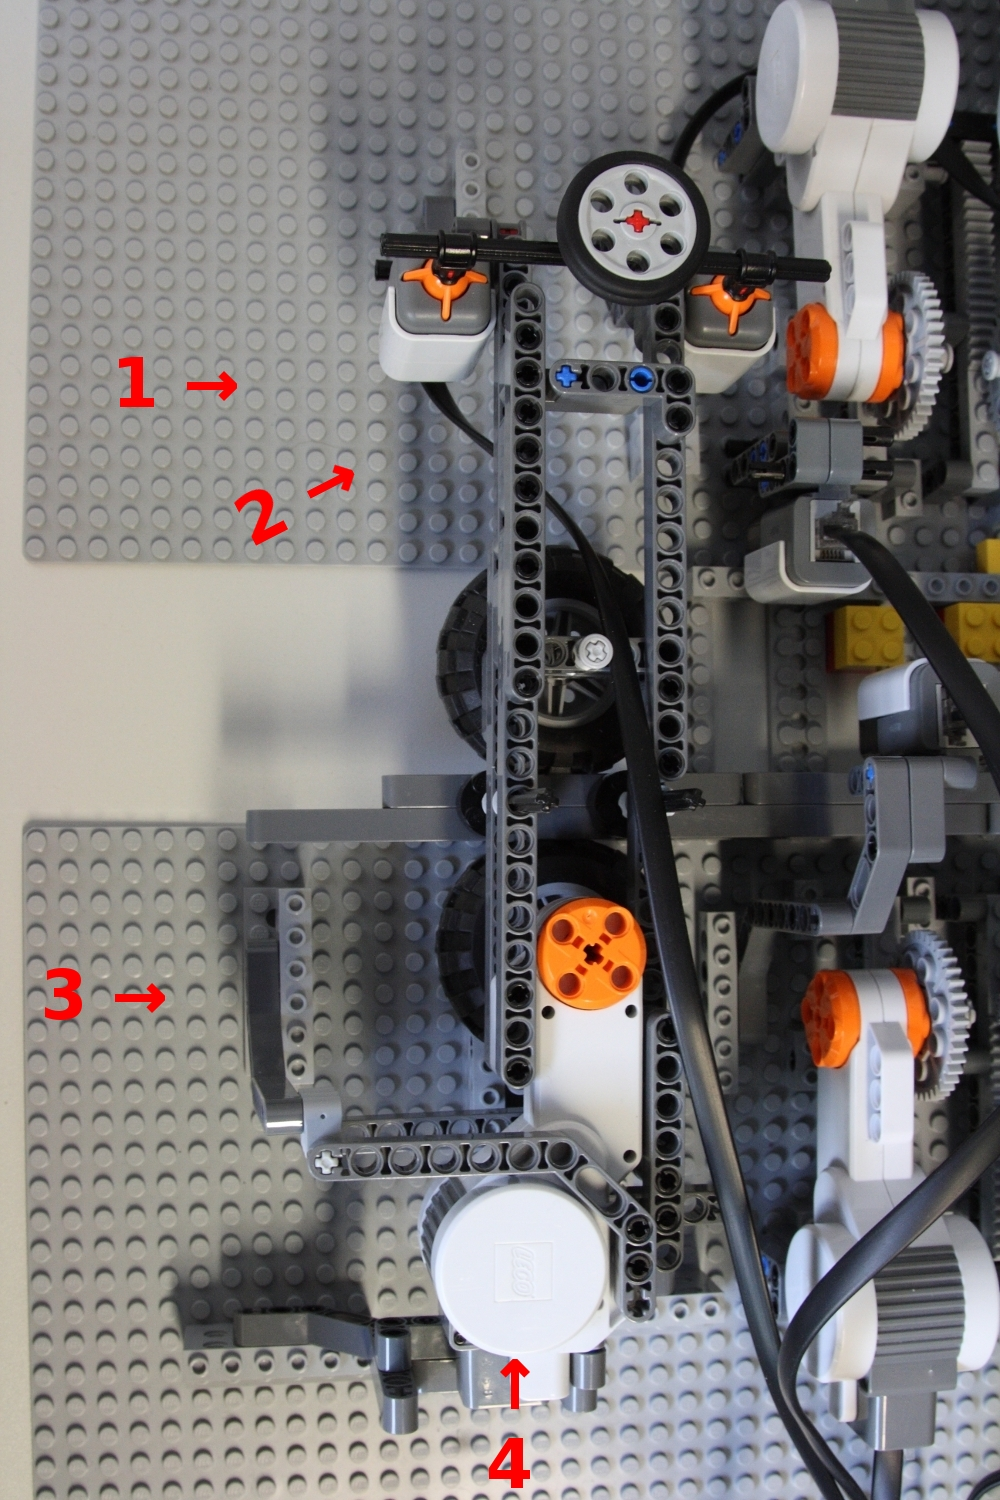
\includegraphics[scale=0.28]{graphics_lego/topview.jpg}
\end{center}
\caption{Overview of the motor section}
\label{pic:topview}
\end{figure}

\clearpage

Figure \ref{pic:position1} shows how the upper left pier has to be placed in relation to the left edge of the upper plate.

\begin{figure}[!htb]
\begin{center}
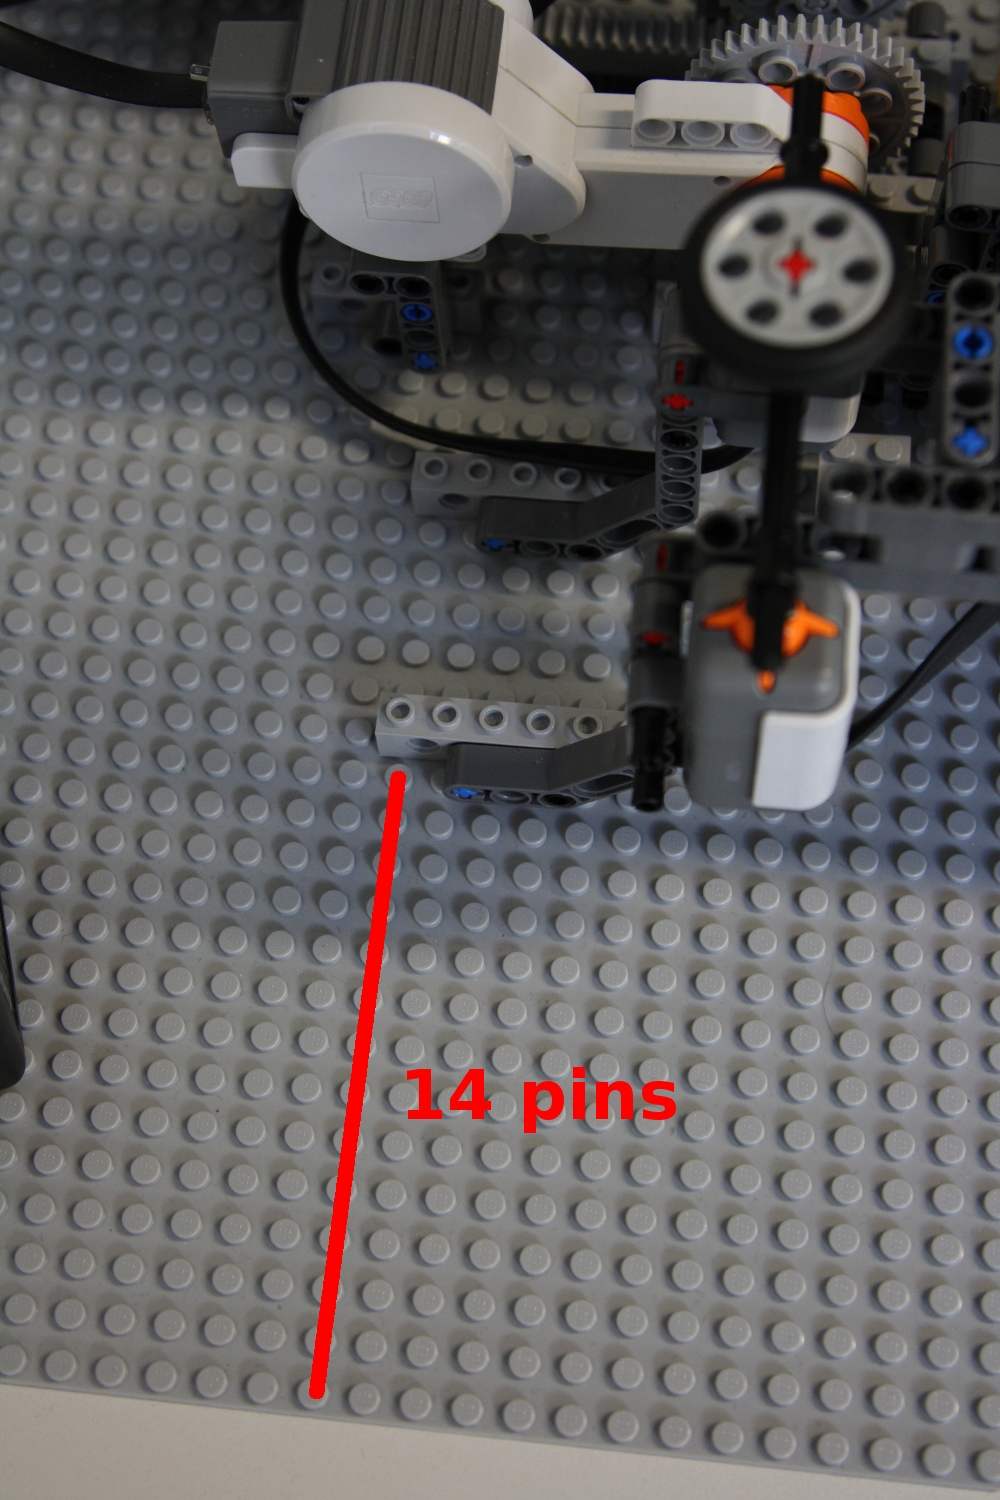
\includegraphics[scale=0.35]{graphics_lego/position1.jpg}
\end{center}
\caption{Image taken from position 1}
\label{pic:position1}
\end{figure}

\clearpage

Figure \ref{pic:position2} shows how the upper left and right pier have to be placed in relation to the bottom edge of the upper plate.

\begin{figure}[!htb]
\begin{center}
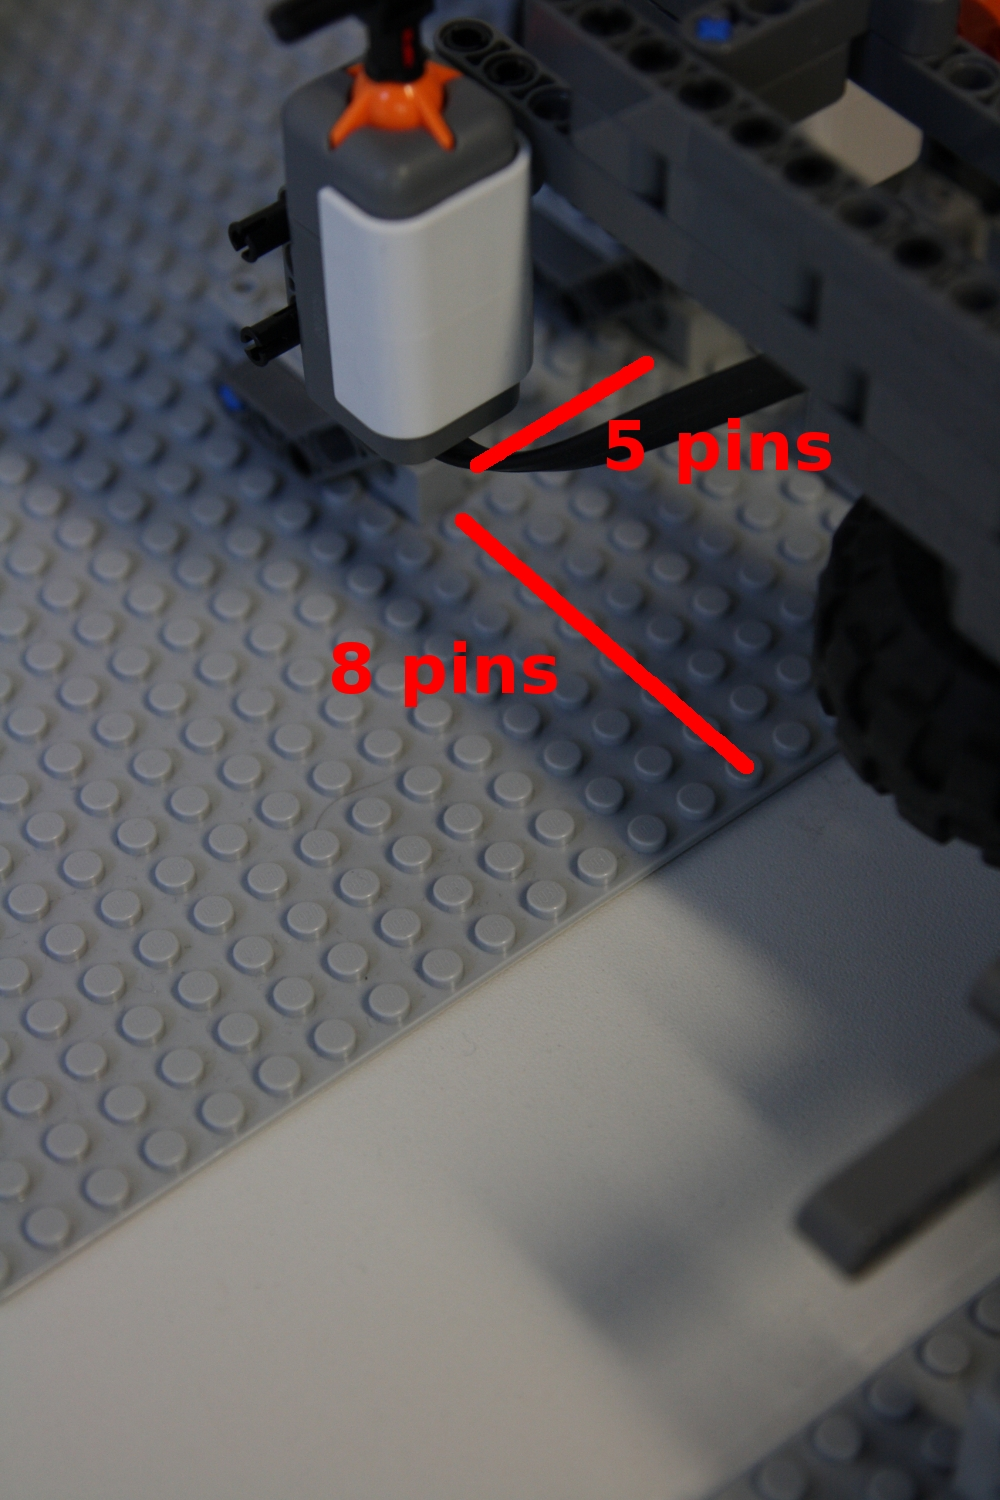
\includegraphics[scale=0.35]{graphics_lego/position2.jpg}
\end{center}
\caption{Image taken from position 2}
\label{pic:position2}
\end{figure}

\clearpage

Figure \ref{pic:position3} shows how the lower left piers have to be placed in relation to the top and left edge of the lower plate.

\begin{figure}[!htb]
\begin{center}
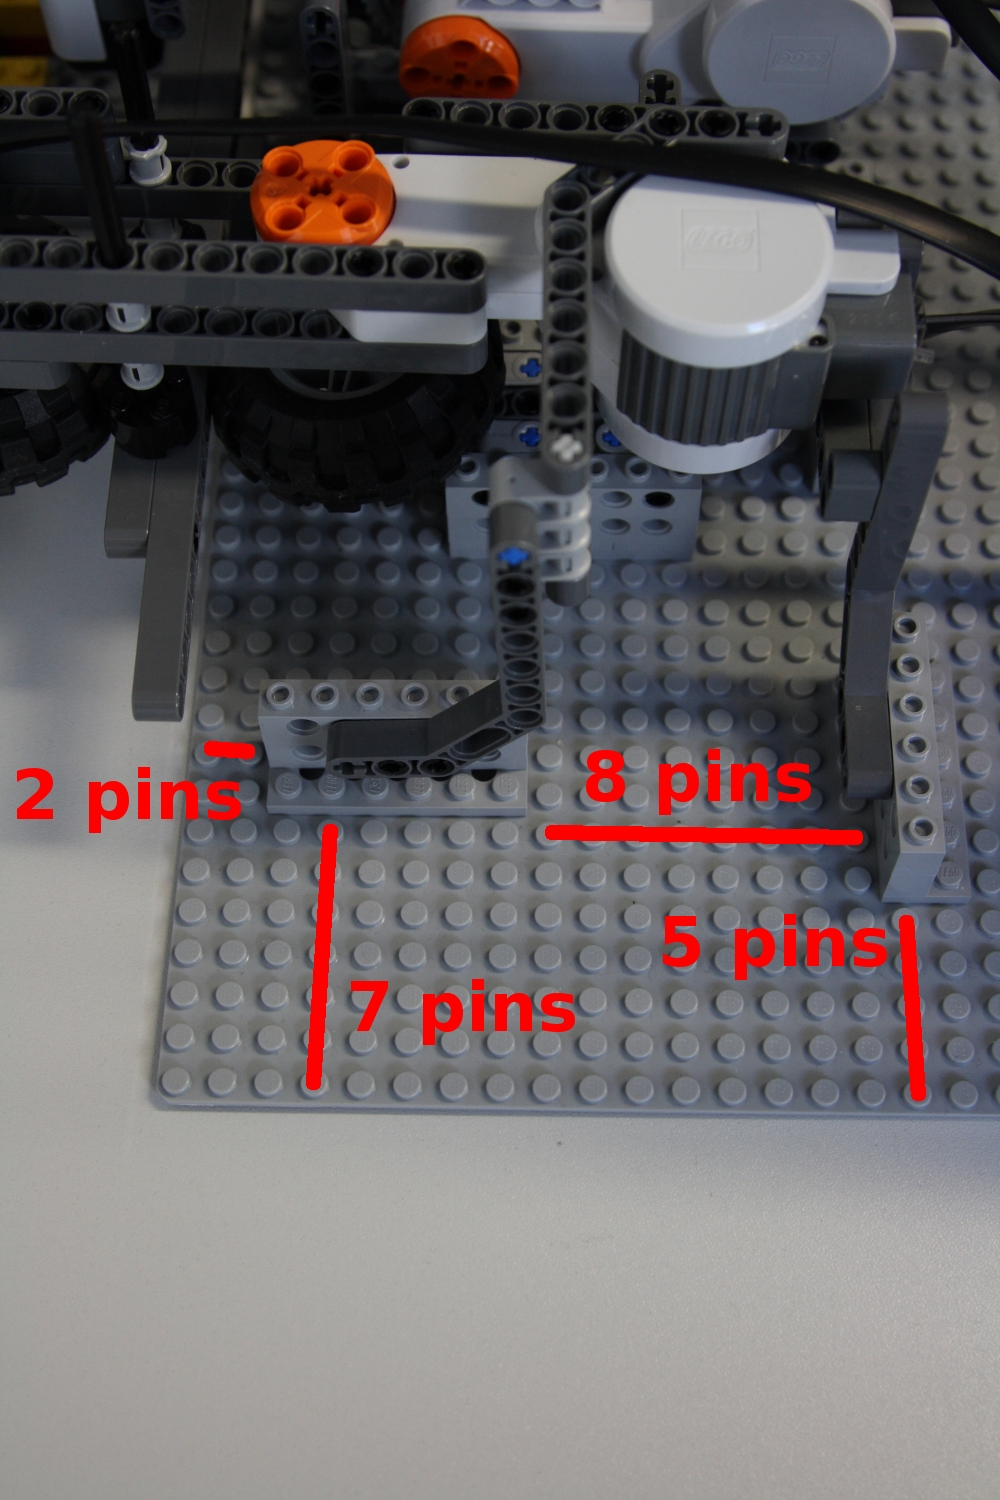
\includegraphics[scale=0.35]{graphics_lego/position3.jpg}
\end{center}
\caption{Image taken from position 3}
\label{pic:position3}
\end{figure}

\clearpage

Figure \ref{pic:position4} shows how the lower right pier has to be placed in relation to the left pier and the support for the motor wheel.

\begin{figure}[!htb]
\begin{center}
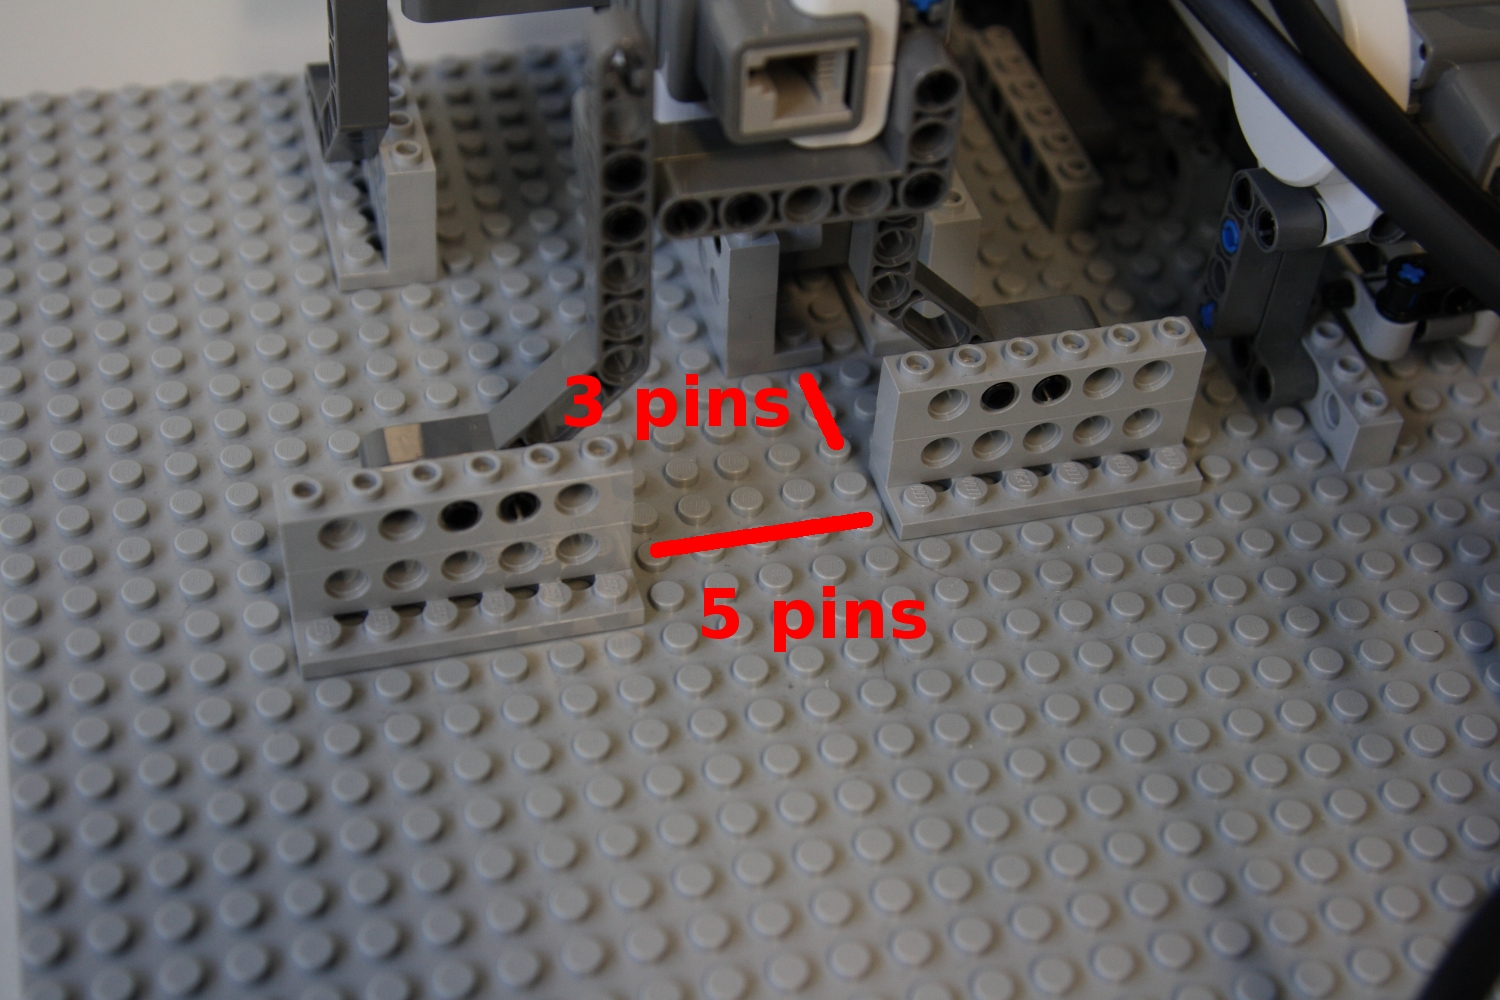
\includegraphics[scale=0.3]{graphics_lego/position4.jpg}
\end{center}
\caption{Image taken from position 4}
\label{pic:position4}
\end{figure}

\clearpage

\subsection{The supporting bridge at the end of the tape}

Figure \ref{pic:bridge2} shows how the upper piers of the supporting bridge have to be placed in relation to the lower and right edge of the upper plate.

\begin{figure}[!htb]
\begin{center}
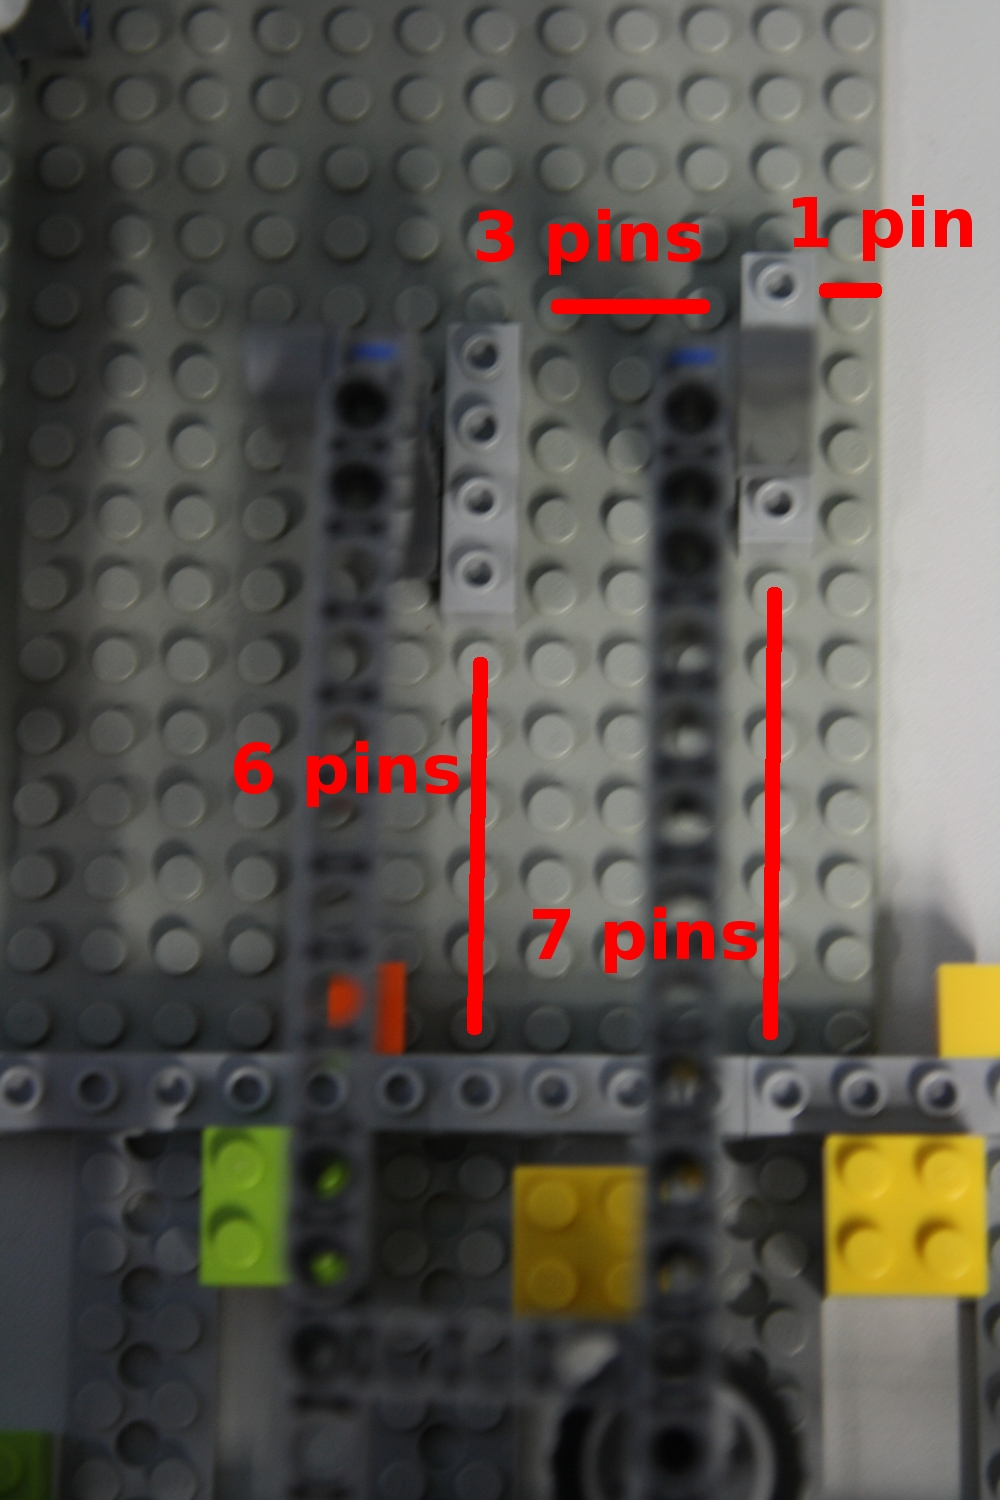
\includegraphics[scale=0.35]{graphics_lego/bridge2.jpg}
\end{center}
\caption{Position of the bridge}
\label{pic:bridge2}
\end{figure}

\clearpage

Figure \ref{pic:bridge1} shows how the lower piers of the supporting bridge have to be placed in relation to the upper and right edge of the lower plate.

\begin{figure}[!htb]
\begin{center}
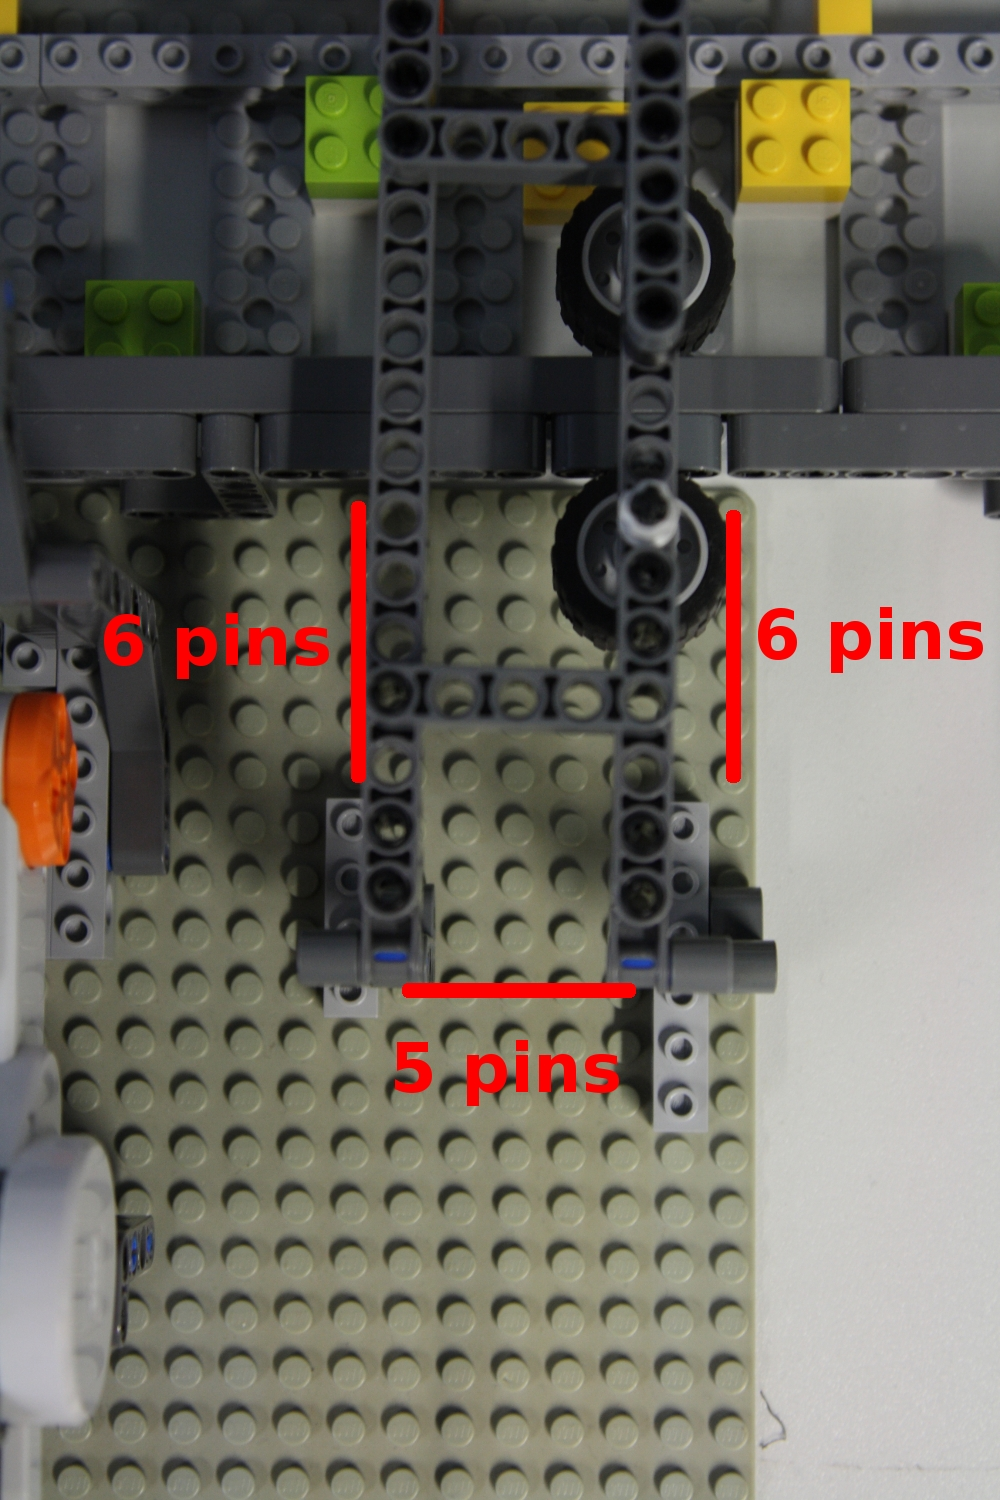
\includegraphics[scale=0.35]{graphics_lego/bridge1.jpg}
\end{center}
\caption{Position of the bridge}
\label{pic:bridge1}
\end{figure}

\clearpage

\subsection{The sensors}

Figure \ref{pic:sensors} shows how the sensors have to be placed to work properly. As you can see the sensor in the rectangle 1 has to be above one of the position bits every time the sensors in rectangle 2 are above two bits at one of the positions.

\begin{figure}[!htb]
\begin{center}
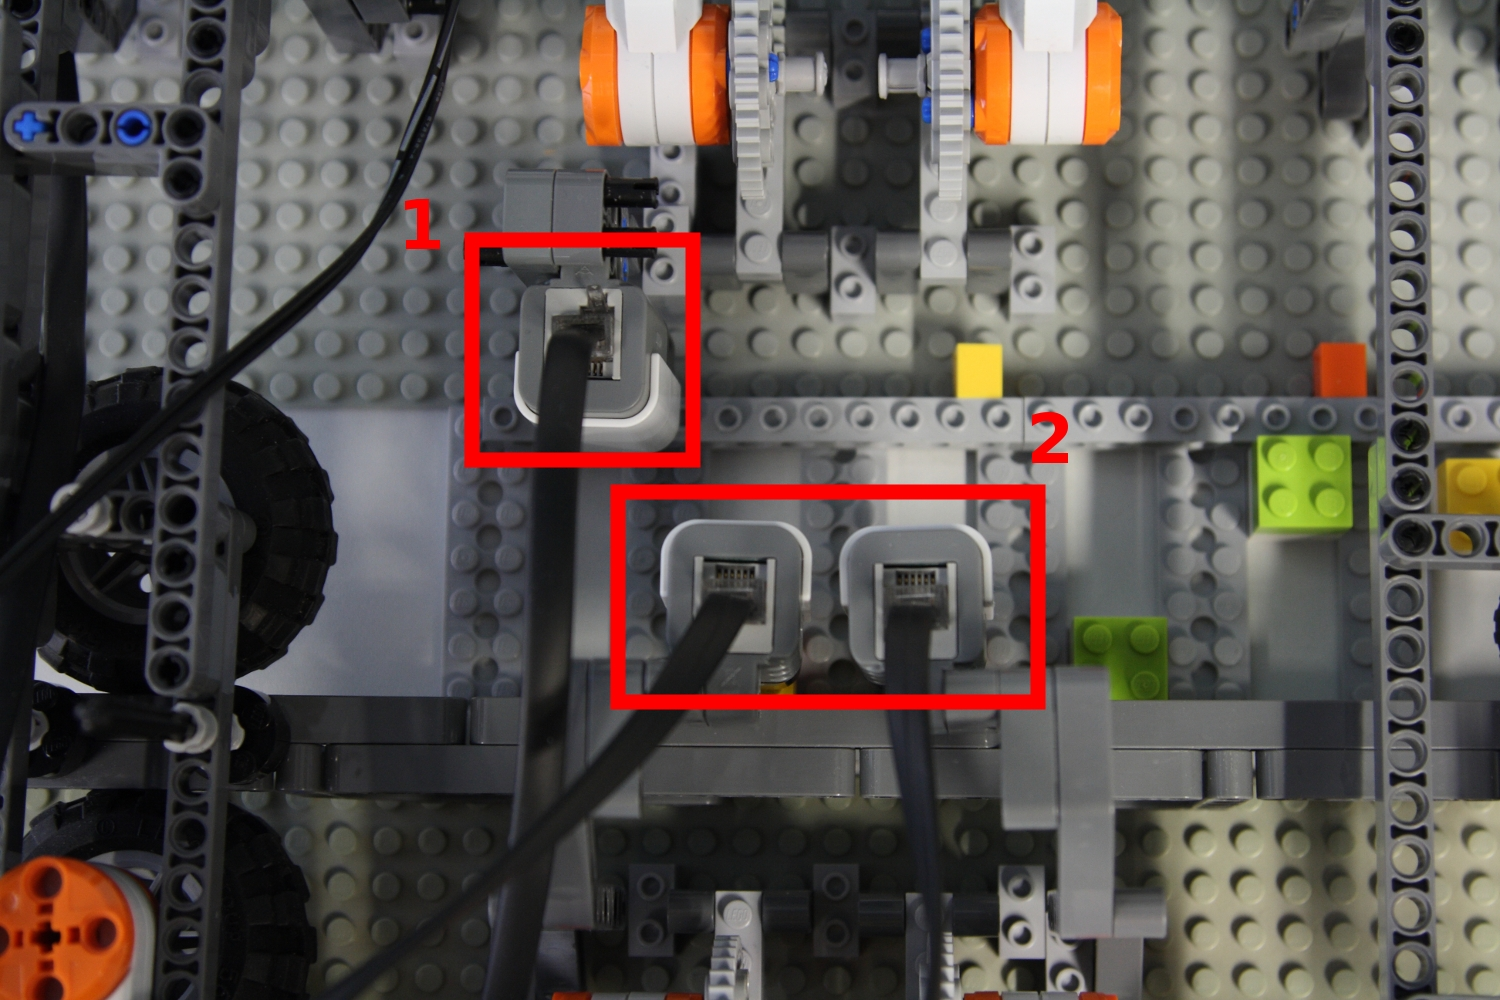
\includegraphics[scale=0.3]{graphics_lego/sensors.jpg}
\end{center}
\caption{Position of the sensors}
\label{pic:sensors}
\end{figure}

\clearpage

\subsection{The tape}

The Marker in Figure \ref{pic:tape} shows how the bricks have to be placed so the sensors recognize them and can distinguish the different positions of the tape. It is also very important that the piers used for the upper bar of the tape are not interfering with the pushers shown in Figure \ref{pic:pusher} and Figure \ref{pic:topview_pushers}. So the pier you can see in the background of Figure \ref{pic:tape} is placed perfectly because it is not preventing the pushers from moving the bits.\\
Here you also can see that 2 bits with the same color always represent one field with a value (\#, 0, 1 or 2).

\begin{figure}[!htb]
\begin{center}
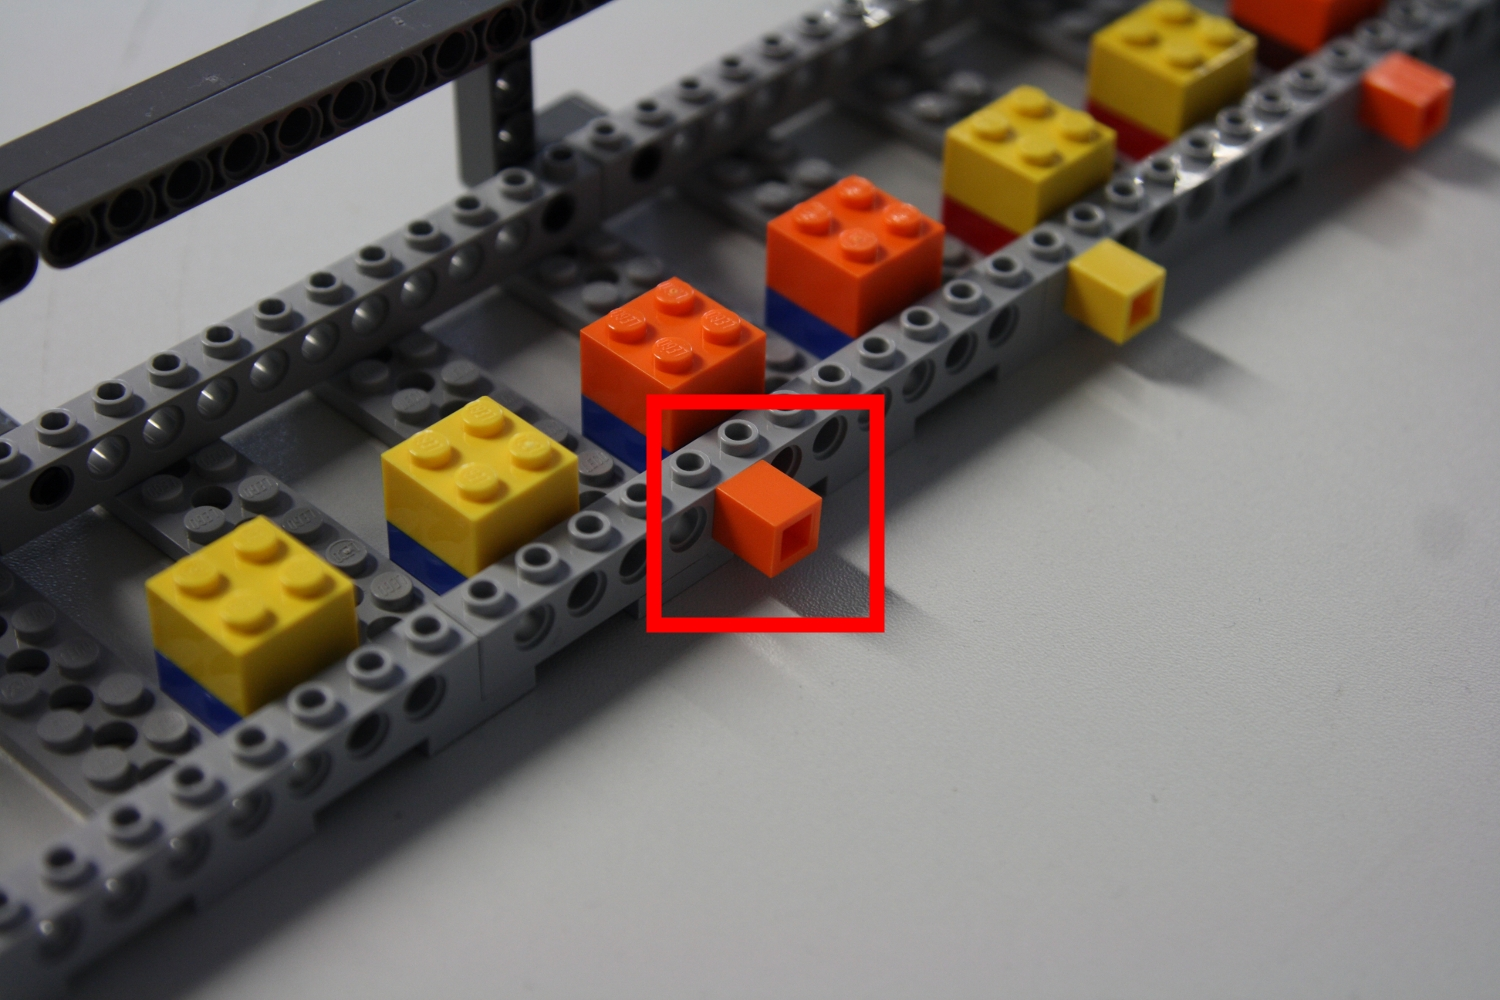
\includegraphics[scale=0.3]{graphics_lego/tape.jpg}
\end{center}
\caption{The tape}
\label{pic:tape}
\end{figure}

\clearpage

Figure \ref{pic:supporting_pier} shows how the supporting piers have to be placed so they do not interfere with the pushers. It also shows how the sensors in the rectangle 2 in figure \ref{pic:sensors} have to be placed so they are above the bits every time the sensor in rectangle 1 is above a position bit.

\begin{figure}[!htb]
\begin{center}
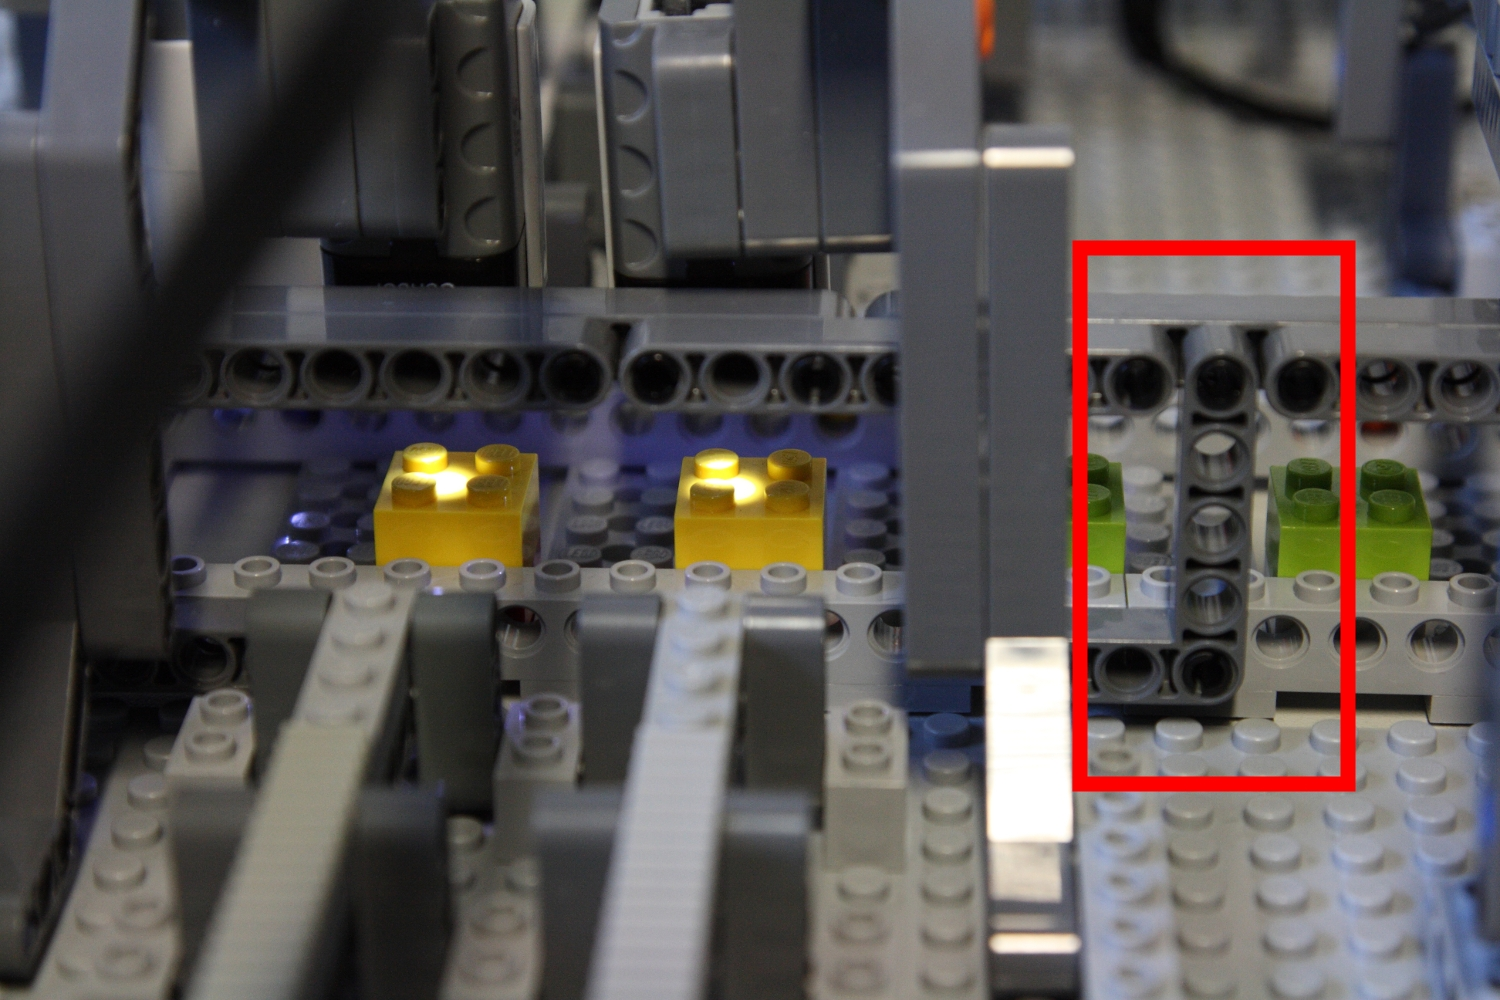
\includegraphics[scale=0.3]{graphics_lego/supporting_pier.jpg}
\end{center}
\caption{One of the supporting piers}
\label{pic:supporting_pier}
\end{figure}

\subsection{Possible bit combinations on the tape}

Figure \ref{pic:bit_combinations} shows all possible legal bit combinations on the tape with their respective value.

\begin{figure}[!htb]
\begin{center}
\begin{tikzpicture}
%\draw[help lines,scale=0.5] (0,0) grid (20,5);
\draw[thick,scale=0.5] (1,1) rectangle +(1,1);
\draw[thick,scale=0.5] (3,1) rectangle +(1,1);
\draw[thick,scale=0.5,fill=tuRed] (1,3) rectangle +(1,1);
\draw[thick,scale=0.5,fill=tuRed] (3,3) rectangle +(1,1);
\draw (1.25,0.25) node[draw=none] {\#};

\draw[thick,scale=0.5] (6,1) rectangle +(1,1);
\draw[thick,scale=0.5,fill=tuRed] (8,1) rectangle +(1,1);
\draw[thick,scale=0.5,fill=tuRed] (6,3) rectangle +(1,1);
\draw[thick,scale=0.5] (8,3) rectangle +(1,1);
\draw (3.75,0.25) node[draw=none] {0};

\draw[thick,scale=0.5,fill=tuRed] (11,1) rectangle +(1,1);
\draw[thick,scale=0.5] (13,1) rectangle +(1,1);
\draw[thick,scale=0.5] (11,3) rectangle +(1,1);
\draw[thick,scale=0.5,fill=tuRed] (13,3) rectangle +(1,1);
\draw (6.25,0.25) node[draw=none] {1};

\draw[thick,scale=0.5,fill=tuRed] (16,1) rectangle +(1,1);
\draw[thick,scale=0.5,fill=tuRed] (18,1) rectangle +(1,1);
\draw[thick,scale=0.5] (16,3) rectangle +(1,1);
\draw[thick,scale=0.5] (18,3) rectangle +(1,1);
\draw (8.75,0.25) node[draw=none] {2};
\end{tikzpicture}
\end{center}
\caption{Bit combinations}
\label{pic:bit_combinations}
\end{figure}

\clearpage

\subsection{The pushers}

Figure \ref{pic:pusher} shows how the pushers have to be placed on the guard rail so they can be pushed properly by the gear wheels. It also shows how the gear wheel has to be placed on the pusher so it pushes properly.

\begin{figure}[!htb]
\begin{center}
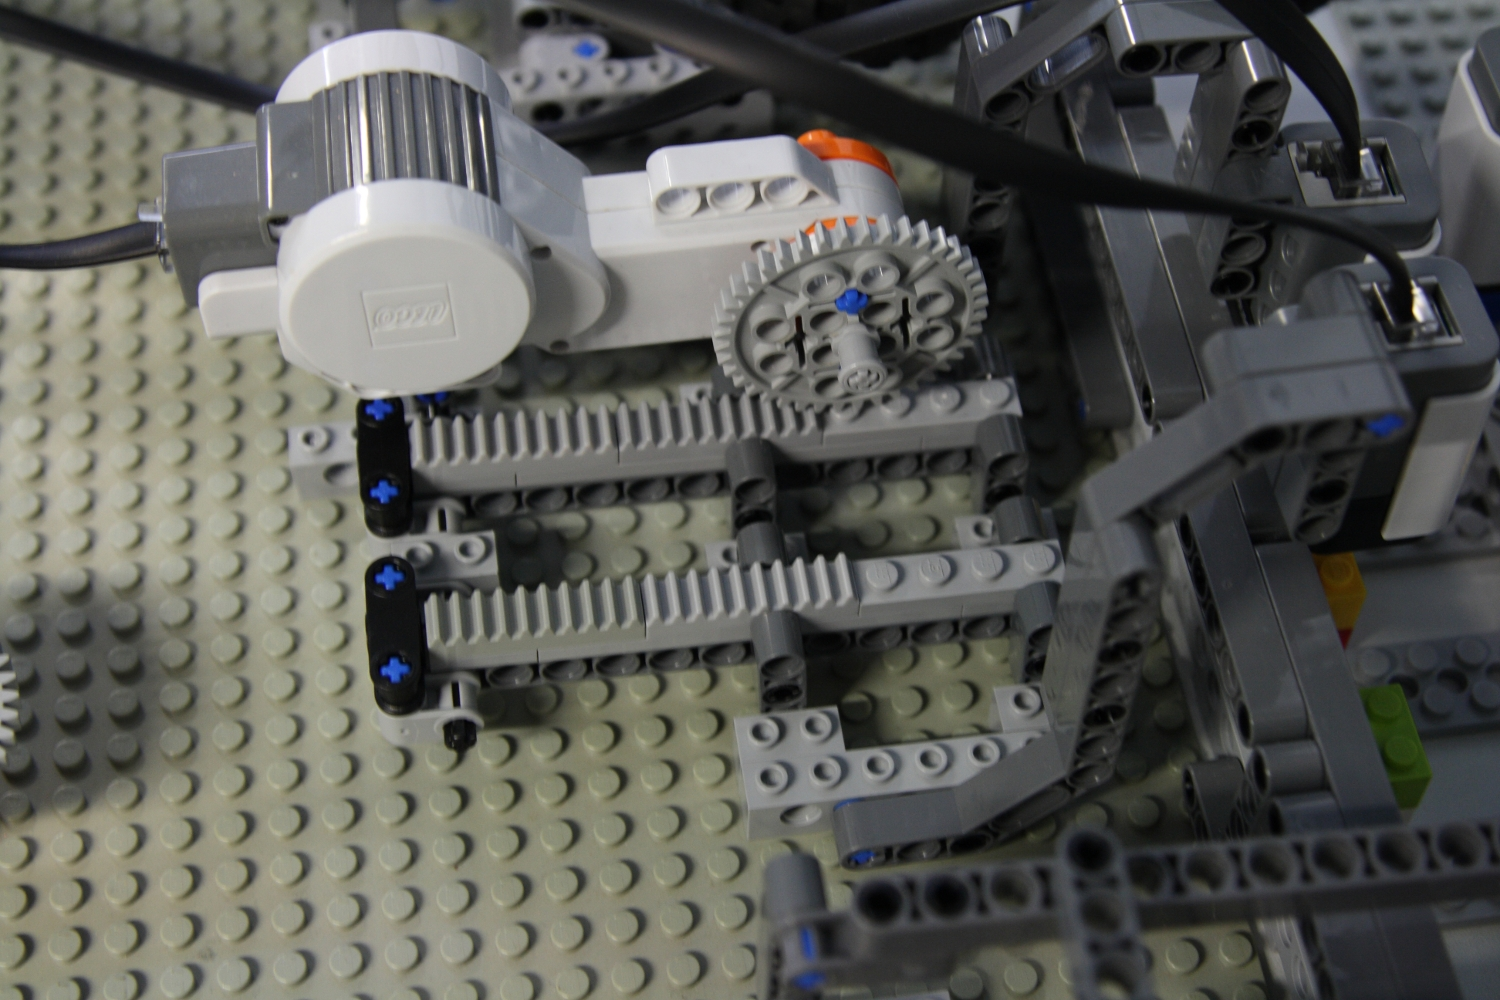
\includegraphics[scale=0.3]{graphics_lego/pusher.jpg}
\end{center}
\caption{Pusher}
\label{pic:pusher}
\end{figure}

\clearpage

Figure \ref{pic:topview_pushers} shows how the pushers are pushing the bits and how to place the supporting piers (rectangle) for the tape's upper bar so they do not interfere with the pushers.

\begin{figure}[!htb]
\begin{center}
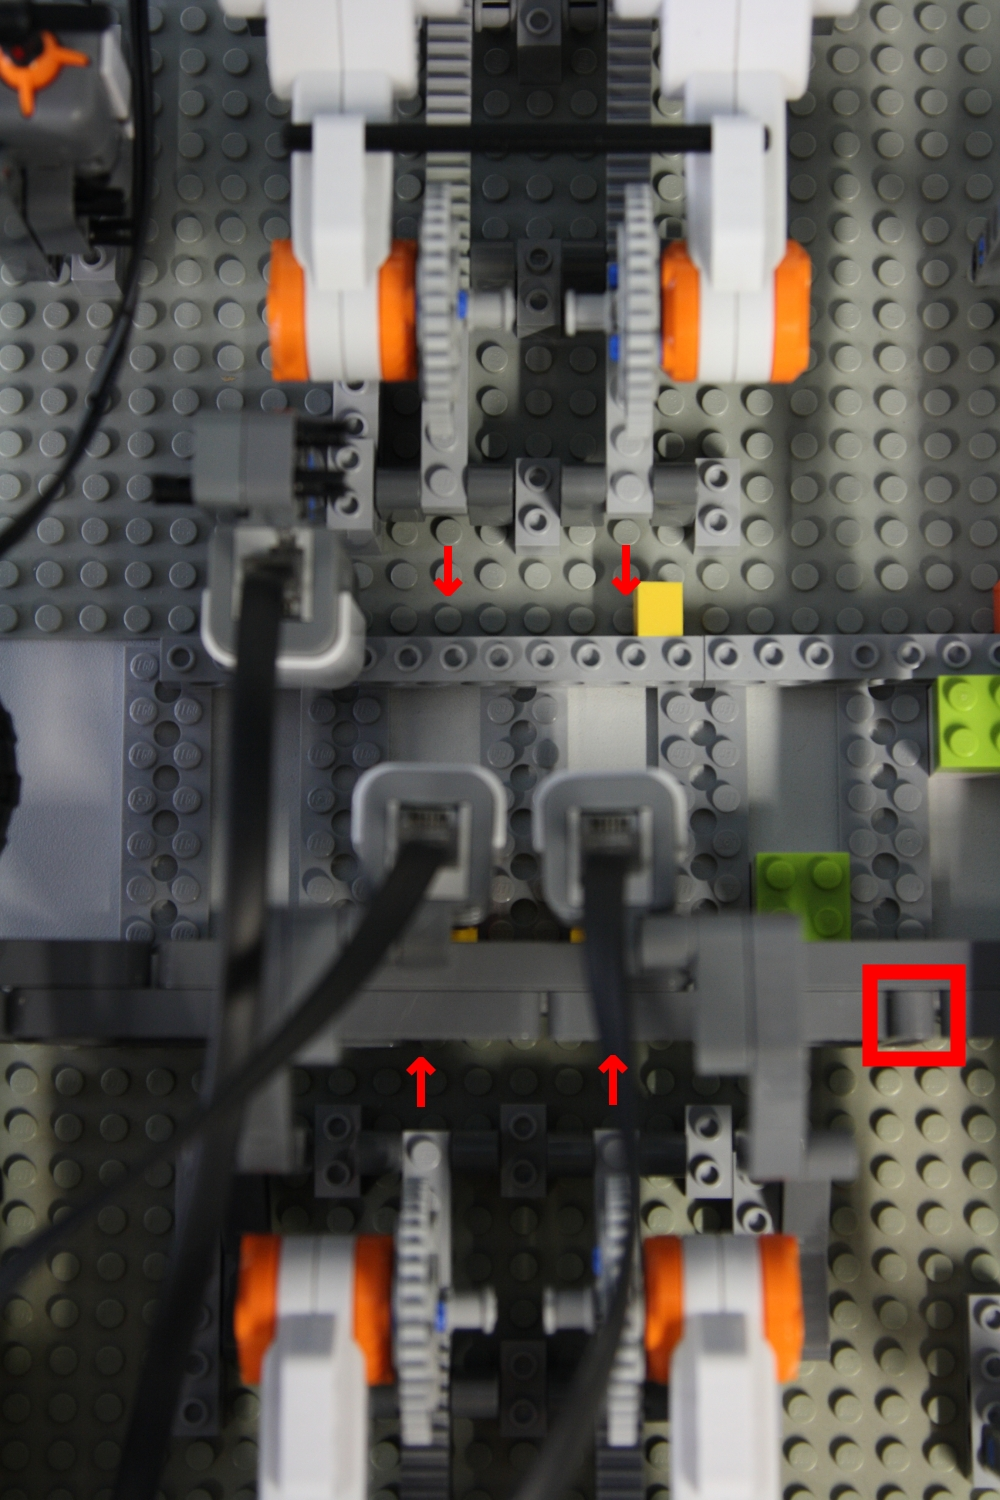
\includegraphics[scale=0.35]{graphics_lego/topview_pushers.jpg}
\end{center}
\caption{Position of the pushers}
\label{pic:topview_pushers}
\end{figure}


\makebackpage[trisec]%[<plain/info/addressinfo>]

\end{document}
